% RePressDB supplementary material
\documentclass[preprint,12pt,authoryear]{elsarticle}
\usepackage{amsmath,amssymb}
\usepackage{booktabs}
\usepackage{tabularx}
\usepackage{threeparttable}
\usepackage{graphicx}
\usepackage{siunitx}
\usepackage{float}
\usepackage{longtable}
\usepackage{seqsplit}
\usepackage{xurl}
\usepackage[hidelinks]{hyperref}
\journal{Journal of Systems and Software}
\biboptions{authoryear,round}
\graphicspath{{./}}
\setlength{\emergencystretch}{2em}
% Auto-generated from frozen CSV/JSON evidence. Do not edit manually.
\newcommand{\EvidenceFreezeVOneFiveOne}{19aad963a625e14c2298bb783bc4885dff062ae17427200f0f1cfbcb7713ed39}
\newcommand{\EvidenceFreezeVOneSevenZero}{ff773467a5de296e07dcbaac904b2d26c466a815ca7b16bdcddbff527a2c4088}
\newcommand{\ReplayRepressShapeRatio}{0.9617}
\newcommand{\ReplayRepressShapeLow}{0.9551}
\newcommand{\ReplayRepressShapeHigh}{0.9689}
\newcommand{\ReplayRepressShapeWins}{18}
\newcommand{\ReplayRepressInitialRatio}{0.9488}
\newcommand{\ReplayRepressInitialLow}{0.9365}
\newcommand{\ReplayRepressInitialHigh}{0.9609}
\newcommand{\ReplayRepressInitialWins}{18}
\newcommand{\ReplayRepressPHRatio}{0.9800}
\newcommand{\ReplayRepressPHLow}{0.9710}
\newcommand{\ReplayRepressPHHigh}{0.9888}
\newcommand{\ReplayRepressPHWins}{15}
\newcommand{\ReplayRepressAFHCRatio}{0.8780}
\newcommand{\ReplayRepressAFHCLow}{0.8439}
\newcommand{\ReplayRepressAFHCHigh}{0.9123}
\newcommand{\ReplayRepressAFHCWins}{18}
\newcommand{\ReplayRepressBestStaticRatio}{1.0564}
\newcommand{\ReplayRepressBestStaticLow}{1.0311}
\newcommand{\ReplayRepressBestStaticHigh}{1.0819}
\newcommand{\ReplayRepressBestStaticWins}{3}
\newcommand{\ReplayRepressMigrations}{185}
\newcommand{\ReplayShapeMigrations}{361}
\newcommand{\ReplayRepressUnamortized}{8.65\%}
\newcommand{\ReplayShapeUnamortized}{70.91\%}
\newcommand{\ReplayRepressStale}{12.43\%}
\newcommand{\ReplayShapeStale}{22.19\%}
\newcommand{\EndToEndQueries}{16,908,066}
\newcommand{\EndToEndPairs}{54}
\newcommand{\EndToEndWorkers}{108}
\newcommand{\EndToEndRepressShapeRatio}{0.9575}
\newcommand{\EndToEndRepressShapeLow}{0.7605}
\newcommand{\EndToEndRepressShapeHigh}{1.2027}
\newcommand{\EndToEndRepressShapeMedian}{1.0009}
\newcommand{\EndToEndRepressInitialRatio}{0.9896}
\newcommand{\EndToEndRepressInitialLow}{0.8379}
\newcommand{\EndToEndRepressInitialHigh}{1.1302}
\newcommand{\EndToEndRepressShapePnnRatio}{1.1256}
\newcommand{\EndToEndRepressShapePnnLow}{0.8470}
\newcommand{\EndToEndRepressShapePnnHigh}{1.5159}
\newcommand{\EndToEndRepressInitialPnnRatio}{1.3803}
\newcommand{\EndToEndRepressInitialPnnLow}{1.0653}
\newcommand{\EndToEndRepressInitialPnnHigh}{1.7535}
\newcommand{\LegacyDiagnosticRepressShape}{1.4142}
\newcommand{\CombinedRecoveryTrials}{1,100}
\newcommand{\CalibrationSeconds}{26.10}
\newcommand{\CalibrationReadMB}{923.23}
\newcommand{\CalibrationWriteMB}{113.15}
\newcommand{\CalibrationCandidateRatio}{3.94}
\newcommand{\CacheInitialServiceRatio}{0.4718}
\newcommand{\CacheInitialServiceLow}{0.3778}
\newcommand{\CacheInitialServiceHigh}{0.6084}
\newcommand{\CacheInitialDispatchRatio}{0.0329}
\newcommand{\CacheInitialPnnRatio}{0.4548}
\newcommand{\CacheShapeServiceRatio}{0.3560}
\newcommand{\CacheShapeServiceLow}{0.3400}
\newcommand{\CacheShapeServiceHigh}{0.3734}
\newcommand{\CacheShapeDispatchRatio}{0.0198}
\newcommand{\CacheShapePnnRatio}{0.3333}
\newcommand{\CacheRepressServiceRatio}{0.2638}
\newcommand{\CacheRepressServiceLow}{0.2168}
\newcommand{\CacheRepressServiceHigh}{0.3316}
\newcommand{\CacheRepressDispatchRatio}{0.0123}
\newcommand{\CacheRepressPnnRatio}{0.3761}

\input{artifact_links.tex}

\begin{document}
\begin{frontmatter}
\title{Supplementary material for ``RePressDB: A Dependable Self-Adaptive Storage Architecture for Nonstationary Time-Series Workloads''}
\author[aff1]{Zhichao Zhang\corref{cor1}}
\ead{zhichao.zhang2024@outlook.com}
\author[aff2]{Xiaolu Peng\fnref{equal2}}
\ead{lilypxl1656179423@outlook.com}
\author[aff1]{Daoqi Sun\fnref{equal2}}
\ead{sundao0217@gmail.com}
\cortext[cor1]{Corresponding author: Zhichao Zhang (zhichao.zhang2024@outlook.com).}
\fntext[equal2]{Xiaolu Peng and Daoqi Sun contributed equally to this work and are co-second authors.}
\address[aff1]{School of Science, Minzu University of China, No. 27 Zhongguancun South Avenue, Beijing, 100081, China}
\address[aff2]{School of Navigation, Dalian Maritime University, No. 1 Linghai Road, Ganjingzi District, Dalian 116026, China}
\end{frontmatter}

\section{Purpose, numerical discipline, and experimental records}

This supplement records the evaluation details, configurations, and supporting measurements used in the study. Result tables are generated from archived CSV or JSON evidence, and derived values are propagated through shared numerical macros. The two archived experiment packages are:

\begin{table}[H]
\centering
\caption{Archived experiment packages.}
\begin{tabularx}{\textwidth}{@{}lX@{}}
\toprule
Evidence package & SHA-256 \\
\midrule
J2/J3/J4 experiment package (v1.5.1) & \begin{minipage}[t]{\linewidth}\ttfamily\scriptsize 19aad963a625e14c2298bb783bc4885d\\ff062ae17427200f0f1cfbcb7713ed39\end{minipage} \\
Paired end-to-end package (v1.7.0) & \begin{minipage}[t]{\linewidth}\ttfamily\scriptsize ff773467a5de296e07dcbaac904b2d26\\c466a815ca7b16bdcddbff527a2c4088\end{minipage} \\
\bottomrule
\end{tabularx}
\end{table}

The v1.5.1 package freezes independently seeded measured-cost replay, unified ablation, randomized termination/corruption, and calibration studies. The v1.7.0 package freezes the paired uncached-versus-active-view end-to-end campaign. Neither package is used to retune RePressDB or Shape-EWMA-BE.

\section{Controller and baseline configurations}

\subsection{RePressDB}

\begin{table}[H]
\centering
\caption{Controller settings.}
\begin{tabularx}{\textwidth}{@{}p{0.34\textwidth}X@{}}
\toprule
Setting & Value \\
\midrule
Long/short windows & 300 / 100 local queries \\
Minimum observations & 200 local queries \\
Decision interval & 100 local queries \\
Confirmation rounds & 3 \\
Cooldown & 300 local queries \\
Projection horizon & 1,200 local queries \\
Minimum relative gain & 8\% \\
Migration safety factor & 1.25 \\
Global budget interval & 1,000 global queries \\
Budget bytes & Largest measured directed rewrite in the corresponding cost table \\
\bottomrule
\end{tabularx}
\end{table}

\subsection{Shape-EWMA-BE and Page-Hinkley-BE}

Shape-EWMA-BE was selected only on the PEMS04 development data. The search contained 80 configurations; 44 passed the pre-registered brief-burst and stable-scan safety gates. The selected configuration was within 0.5\% of the best action score and minimized migrations and rewritten bytes within that equivalence set.

\begin{table}[H]
\centering
\caption{Baseline configurations.}
\begin{tabularx}{\textwidth}{@{}lX@{}}
\toprule
Baseline & Configuration and runtime information \\
\midrule
Shape-EWMA-BE & EWMA $\alpha=0.01$, relative deadband $0.05$, horizon 300, decision interval 100, minimum observations 200, and measured directed break-even. It observes only past query classes. \\
Page-Hinkley-BE & Page-Hinkley $\delta=0.005$, threshold 10, window cap 300, deadband $0.05$, horizon 600, and the same measured directed break-even. It observes only past query classes. \\
AF-HC-D & Access-frequency hot/cold detector with a deadband and the same write budget; decisions use access frequency instead of the eight-class query-shape monitor. \\
Initial-best & Deployable static representation chosen for the fixed initial scan-heavy mixture. \\
Best-static & Nondeployable hindsight reference selected from the complete trace with a free initial choice. \\
Migration-aware oracle & Nondeployable future-aware reference that sees phase boundaries and future duration. \\
\bottomrule
\end{tabularx}
\end{table}

\section{Multi-seed measured-cost replay}

The statistical unit is one independently generated trace realization fixed before policy execution. The campaign contains three trace families, two sizes, and three pre-registered seeds, giving 18 realization-level cells. Ratios use equal-weight geometric means. Query and directed migration costs use file-backed medians from the archived calibration tables; system-level timing is measured separately in the paired file-backed campaign.

\begin{table}[H]
\centering
\caption{Multi-seed replay results.}
\resizebox{\textwidth}{!}{%
\begin{tabular}{@{}lrrrrrr@{}}
\toprule
Trace & Size & RePress/Shape & RePress/initial & RePress/PH-BE & RePress mig. & Shape mig. \\
\midrule
Gradual-periodic & 8K & 0.9453 & 0.9453 & 0.9590 & 44 & 0 \\
Gradual-periodic & 16K & 0.9586 & 0.9067 & 0.9956 & 55 & 40 \\
Mean-reverting & 8K & 0.9806 & 0.9806 & 1.0008 & 6 & 0 \\
Mean-reverting & 16K & 0.9541 & 0.9355 & 0.9624 & 41 & 170 \\
Noisy bursts & 8K & 0.9795 & 0.9795 & 0.9986 & 6 & 0 \\
Noisy bursts & 16K & 0.9527 & 0.9472 & 0.9648 & 33 & 151 \\
\midrule
All cells & N/A & 0.9617 & 0.9488 & 0.9800 & 185 & 361 \\
\bottomrule
\end{tabular}}
\end{table}

Across all 18 cells, RePressDB/Shape-EWMA-BE is \ReplayRepressShapeRatio{} (bootstrap 95\% CI \ReplayRepressShapeLow-\ReplayRepressShapeHigh), and RePressDB is lower in \ReplayRepressShapeWins{}/18 cells. RePressDB/initial-best is \ReplayRepressInitialRatio, RePressDB/Page-Hinkley-BE is \ReplayRepressPHRatio{} with 15/18 lower cells, and RePressDB/free best-static is \ReplayRepressBestStaticRatio. Best-static has complete-trace knowledge and a free initial choice, so this comparison is interpreted as an optimistic offline reference.

\begin{table}[H]
\centering
\caption{Aggregate migration-risk results.}
\begin{tabular}{@{}lrrr@{}}
\toprule
Policy & Migrations & Unamortized rate & Stale rate \\
\midrule
AF-HC-D & 997 & 66.90\% & 43.70\% \\
Page-Hinkley-BE & 708 & 71.89\% & 30.96\% \\
Shape-EWMA-BE & \ReplayShapeMigrations{} & \ReplayShapeUnamortized{} & \ReplayShapeStale{} \\
RePressDB & \ReplayRepressMigrations{} & \ReplayRepressUnamortized{} & \ReplayRepressStale{} \\
\bottomrule
\end{tabular}
\end{table}

\section{Unified component ablation}

The six variants use the same plans, profiles, migration matrices, and write-budget accounting. The ablation is interpreted through the joint behavior of replay cost, migration count, and migration-risk measures.

\begin{table}[H]
\centering
\caption{Ablation results.}
\resizebox{\textwidth}{!}{%
\begin{tabular}{@{}lrrrrr@{}}
\toprule
Variant & Cost ratio & 95\% CI & Migrations & Median unamortized & Median stale \\
\midrule
Full RePressDB & 1.0000 & [1.0000, 1.0000] & 66 & 3.33\% & 2.78\% \\
No break-even & 0.9667 & [0.9428, 0.9886] & 130 & 16.23\% & 16.23\% \\
No confirmation & 0.9857 & [0.9600, 1.0102] & 229 & 10.51\% & 0.00\% \\
No cooldown & 1.0000 & [1.0000, 1.0000] & 66 & 3.33\% & 2.78\% \\
No write budget & 0.9994 & [0.9988, 0.9999] & 66 & 3.33\% & 2.78\% \\
Short-window only & 0.9941 & [0.9803, 1.0073] & 126 & 8.33\% & 2.63\% \\
\bottomrule
\end{tabular}}
\end{table}

Removing break-even changes replay cost to 0.9667 of full RePressDB while migrations increase from 66 to 130 and the median unamortized rate increases from 3.33\% to 16.23\%. Removing confirmation raises migrations to 229. In these six cells, cooldown and the write-budget constraint are activated infrequently enough that aggregate cost and migration count remain close to full RePressDB; their role is to bound temporal reversals and aggregate write activity.

\subsection{Clean-stage responsiveness holdout}
The clean-stage holdouts isolate response under abrupt, persistent changes. Shape-EWMA-BE reacts earlier to these transitions, while RePressDB performs fewer migrations and rewrites fewer bytes across the same PEMS08 and BDG2 cells. The figure reports both sides of this responsiveness/selectivity trade-off.

\begin{figure}[H]
\centering
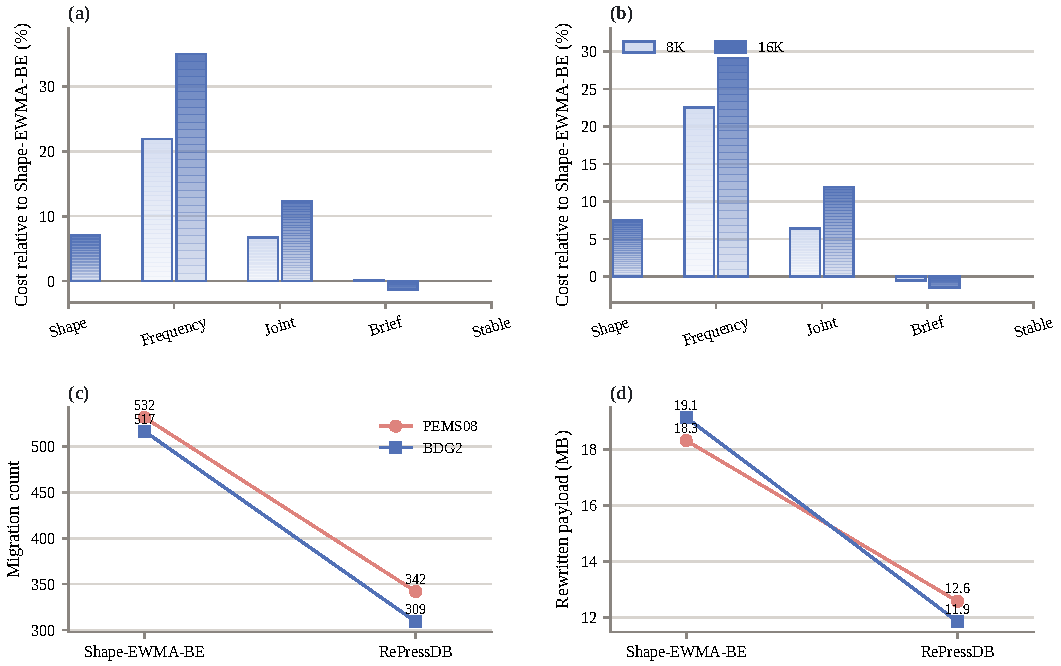
\includegraphics[width=0.98\textwidth]{Figure_3_strong_baseline_tradeoff.pdf}
\caption{Clean-stage holdout results.}
\end{figure}

\section{Paired end-to-end campaign}

\subsection{Process structure and pairing}

The v1.7.0 launcher retains only Python standard-library modules. It starts one heavy worker, waits for it to exit, and starts the next worker only after the preceding process has released its NumPy, Pandas, codec, SQLite, and result state. The campaign contains \EndToEndPairs{} paired units and \EndToEndWorkers{} isolated workers. Each pair shares trace, size, repeat, policy, calibration table, initial store snapshot, and query realization. Uncached-first and active-view-first orders are balanced 27/27. The total measured query count is \EndToEndQueries, and every query is checked against an independent \texttt{float32} truth array.

Each worker performs one verification query per active chunk before the timed region. This loads the current representation and metadata and matches the \texttt{warm\_slicedmeta} calibration regime. The prewarm cost is reported separately. A post-migration active-view reload remains inside the measured interval.

\begin{table}[H]
\centering
\caption{Active-view execution effect.}
\resizebox{\textwidth}{!}{%
\begin{tabular}{@{}lrrrrrr@{}}
\toprule
Policy & Service ratio & 95\% CI & Dispatch ratio & p99 ratio & Cached faster & Pairs \\
\midrule
Initial-best & 0.4718 & [0.3778, 0.6084] & 0.0329 & 0.4548 & 16/18 & 18 \\
Shape-EWMA-BE & 0.3560 & [0.3400, 0.3734] & 0.0198 & 0.3333 & 18/18 & 18 \\
RePressDB & 0.2638 & [0.2168, 0.3316] & 0.0123 & 0.3761 & 17/18 & 18 \\
\bottomrule
\end{tabular}}
\end{table}

\subsection{Read-path ablation}

\begin{table}[H]
\centering
\caption{Read-path reconstruction counts.}
\begin{tabular}{@{}lrr@{}}
\toprule
Counter & Uncached & Active view \\
\midrule
Catalog-row loads & 16,909,113 & 246 \\
\texttt{StoredChunk} builds & 8,454,711 & 246 \\
Block-metadata parses & 2,358,417 & 246 \\
\bottomrule
\end{tabular}
\end{table}

The uncached path yields a RePressDB/Shape service-time ratio of \LegacyDiagnosticRepressShape. Its accumulated time decomposition is 117.10 versus 106.98 s for codec execution, 186.28 versus 105.31 s for catalog/dispatch, 5.22 versus 6.91 s for controller work, and 2.23 versus 1.14 s for migration work. Repeated catalog and metadata reconstruction account for most of the additional read-path work.

All 54 uncached/active-view pairs have identical migration signatures: event index, chunk, source codec, target codec, and rewrite bytes. Active-view workers incur 93 RePressDB, 30 Shape, and zero initial-best measured cache misses, exactly matching the committed migration counts. The paired design therefore isolates the read-path mechanism while keeping adaptation decisions fixed.

\subsection{Policy comparison with active-view execution}

\begin{table}[H]
\centering
\caption{Policy ratios with active-view execution.}
\resizebox{\textwidth}{!}{%
\begin{tabular}{@{}lrrrr@{}}
\toprule
Comparison & Service ratio & 95\% CI & Median & Wins \\
\midrule
RePressDB / Shape-EWMA-BE & \EndToEndRepressShapeRatio{} & [\EndToEndRepressShapeLow, \EndToEndRepressShapeHigh] & \EndToEndRepressShapeMedian{} & 9/18 \\
RePressDB / initial-best & \EndToEndRepressInitialRatio{} & [\EndToEndRepressInitialLow, \EndToEndRepressInitialHigh] & 1.1014 & 4/18 \\
\bottomrule
\end{tabular}}
\end{table}

The aggregate service-time ratios remain close across the adaptive policies. RePressDB/Shape p99 is \EndToEndRepressShapePnnRatio{} (95\% CI: \EndToEndRepressShapePnnLow--\EndToEndRepressShapePnnHigh), and RePressDB/initial-best p99 is \EndToEndRepressInitialPnnRatio{} (95\% CI: \EndToEndRepressInitialPnnLow--\EndToEndRepressInitialPnnHigh). Three paired units contain large codec-time observations; they remain in every aggregate and confidence interval.

\section{Recovery campaign and state coverage}

\begin{table}[H]
\centering
\caption{Randomized recovery campaign.}
\begin{tabular}{@{}lr@{}}
\toprule
Trial class or pre-termination state & Count \\
\midrule
Abrupt termination: \texttt{idle} & 110 \\
Abrupt termination: \texttt{intent} & 84 \\
Abrupt termination: \texttt{encoded} & 23 \\
Abrupt termination: \texttt{validated} & 31 \\
Abrupt termination: \texttt{published} & 28 \\
Abrupt termination: \texttt{committed\_pending\_cleanup} & 24 \\
Post-commit payload truncation & 75 \\
Post-commit metadata corruption & 50 \\
Orphan staging/final files & 75 \\
\midrule
Randomized campaign total & 500 \\
Earlier controlled protocol-boundary trials & 600 \\
Combined tested trials & \CombinedRecoveryTrials{} \\
\bottomrule
\end{tabular}
\end{table}

All 500 randomized trials finish with a valid idle catalog, exact full-array equality, 20 correct spot queries, no temporary file, no invalid active chunk, no non-idle row, and exactly one active payload. Together with the earlier 600 controlled boundary trials, all \CombinedRecoveryTrials{} completed trials satisfy the recorded recovery and query-correctness checks. The evaluated fault model covers process interruption and selected corruption conditions. Hardware-level power interruption and storage write reordering belong to a stronger durability campaign.

\section{Calibration overhead and robustness}

Fresh calibration covers 64 chunks, five codecs, eight query classes, 2,560 query-cost records, 320 codec records, and 1,600 source-to-target entries. The last count includes five no-op diagonal entries per chunk; there are 20 nontrivial directed migrations per chunk.

\begin{table}[H]
\centering
\caption{Calibration overhead.}
\begin{tabular}{@{}lr@{}}
\toprule
Metric & Value \\
\midrule
Wall time & \CalibrationSeconds{} s \\
CPU user/system & 8.31 / 5.39 s \\
Process reads & \CalibrationReadMB{} MB \\
Process writes & \CalibrationWriteMB{} MB \\
Raw chunk bytes & 3.15 MB \\
Candidate storage & 12.40 MB \\
Candidate/raw ratio & \CalibrationCandidateRatio{}$\times$ \\
\bottomrule
\end{tabular}
\end{table}

\begin{table}[H]
\centering
\caption{Sampled-profile evaluation.}
\resizebox{\textwidth}{!}{%
\begin{tabular}{@{}lrrr@{}}
\toprule
Sample fraction & RePressDB true-cost ratio & Shape true-cost ratio & Median migration Jaccard (RePressDB) \\
\midrule
10\% & 1.0859 & 1.0675 & 0.000 \\
25\% & 1.0835 & 1.0433 & 0.073 \\
50\% & 1.0938 & 1.0265 & 0.131 \\
\bottomrule
\end{tabular}}
\end{table}

A population-median profile built from a subset of chunks changes chunk-specific migration decisions. Independent bounded perturbations of the existing per-chunk cost entries have much smaller effects: at $\pm20\%$, RePressDB's geometric-mean true-cost ratio is 1.0004 and its p95 ratio is 1.0069. These two sensitivity studies separate loss of chunk-specific structure from bounded local measurement error.

\begin{figure}[H]
\centering
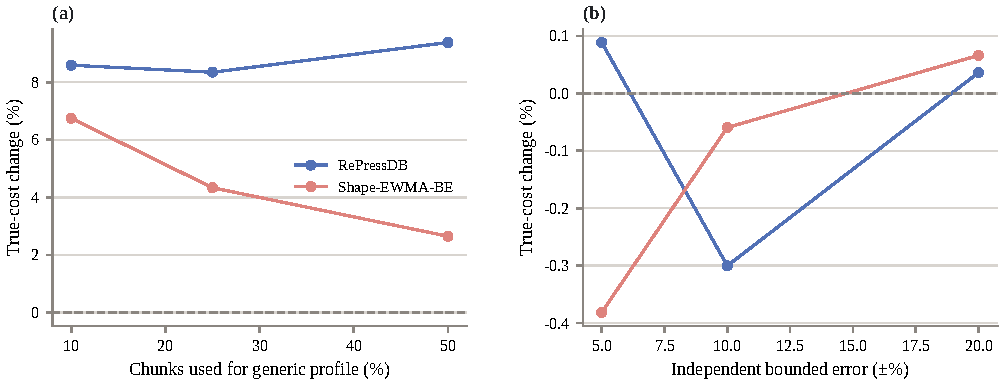
\includegraphics[width=0.96\textwidth]{Figure_10_recovery_calibration.pdf}
\caption{Calibration sensitivity.}
\end{figure}

\section{Physical corpus, logical scale, and interference}

The full cleaned-BDG2 physical campaign contains 564 eligible series, 720 complete 8K chunks, and 3,283 2K catalog chunks. It completes one million verified file queries and 1,000 migrations. This physical campaign is distinct from the shared-template logical-scale experiment.

\begin{table}[H]
\centering
\caption{Logical catalog scaling.}
\resizebox{\textwidth}{!}{%
\begin{tabular}{@{}lrrrrr@{}}
\toprule
Logical scale & Chunks & Tenants & Catalog B/chunk & Clean start (s) & One-dirty-row start (s) \\
\midrule
1 GiB & 32,768 & 46 & 301.5 & 0.283 & 0.317 \\
5 GiB & 163,840 & 228 & 298.6 & 2.656 & 2.958 \\
10 GiB & 327,680 & 456 & 300.5 & 5.526 & 6.190 \\
\bottomrule
\end{tabular}}
\end{table}

The 10-GiB label denotes a logical catalog and routing view over 327,680 chunks backed by shared physical templates. Across nine logical-scale/thread strata, the counterbalanced background-migration campaign gives an aggregate foreground-throughput ratio of 0.9764 and a p99 amplification of 1.0569. Each background cell contains a bounded burst of 50 copy-on-write migrations.

\section{Captured environment and reproducibility details}

\begin{table}[H]
\centering
\caption{Experimental environment.}
\begin{tabularx}{\textwidth}{@{}lX@{}}
\toprule
Item & Captured value \\
\midrule
Operating system/filesystem & Microsoft Windows 11 Home, build 26200; NTFS \\
Processor & Intel Core i7-14700HX; 20 physical cores / 28 logical processors \\
Memory & 16,873,545,728 bytes (16.87 GB; about 15.7 GiB) \\
Storage & YMTC YMSS2ED08D25MC; 1.024 TB; NVMe; firmware LN3603D1 \\
Python & 3.10.20 \\
NumPy / Pandas & 2.2.6 / 2.3.3 \\
SQLite & 3.53.1; WAL; \texttt{synchronous=FULL} \\
LZ4 / Zstandard & 4.4.5 / 0.25.0; whole Zstandard level 3 \\
Data type & Little-endian \texttt{float32} \\
Timer & \texttt{time.perf\_counter\_ns} \\
End-to-end process model & Standard-library launcher; one isolated heavy process per worker; no additional memory-pressure allocation \\
\bottomrule
\end{tabularx}
\end{table}

A same-host hardware capture records the processor and project-drive identifiers reported above. Absolute latency and throughput remain machine-specific. The principal conclusions therefore rely on balanced paired ratios, confidence intervals, medians, and win counts.

\section{Artifact layout and interpretation scope}

The public repository at \href{\ArtifactRepositoryURL}{\ArtifactRepositoryURLText} contains source code, environment records, selection manifests, archived summaries, and generation scripts. Versioned archives distributed through \href{\ArtifactReleaseURL}{\ArtifactReleaseURLText} add all 108 worker summaries, raw latency arrays, recovery and calibration records, and SHA-256 manifests. Public source datasets remain available from their cited repositories.

Measured-cost replay and wall-clock execution are reported separately throughout the study. End-to-end results use the warm-metadata active-view path and balanced paired units. The 10-GiB scale experiment concerns catalog and routing behavior over shared immutable templates. Recovery evidence covers the specified process-interruption and corruption model, with stronger hardware-level durability conditions treated as a separate validation layer. The representation space contains five lossless layouts, and the evaluation uses one file-backed host with real sensor values and controlled or semi-synthetic query flows.

\end{document}
